%=== CHAPTER TWO (2) ===
%=== Literature Review ===

\chapter{Literature Review}
\begin{spacing}{2.0}
%\setlength{\parskip}{0.2in}

\section{Overview}

In chess, the concept of "perfect play" involves making the best possible move that leads to the best possible outcome at every turn [22]. However, determining perfect play requires knowledge of all available moves, a task that is beyond the current capabilities of most chess engines. To attempt perfect play, engines use algorithms such as the min-conflicts algorithm, which iterates through all possible nodes one step at a time to solve the current problem \cite{modernApproach}. However, the computational power required for this limits the engine's ability to process complicated chess positions with numerous possible moves, leading to enforced time limits depending on the match's time controls.

In 2018, Bojun Guo and Ronald de Man completed the first publicly available free 7-piece tablebase, a database of all possible moves and outcomes for positions involving seven or fewer chess pieces on the board\footnote{\url{https://lichess.org/blog/W3WeMyQAACQAdfAL/7-piece-syzygy-tablebases-are-complete}} With the use of this tablebase, engines are able to play perfectly when there are only 7 chess pieces left on the board. This has significantly improved the engines' ability to play at a high level, and has opened up new possibilities for computer chess research.

While perfect play remains a lofty goal for chess engines, the development of tablebases such as the 7-piece tablebase marks a significant step forward in their ability to achieve it. As computational power and algorithms continue to improve, we may eventually see chess engines capable of perfect play even in the most complex of positions.
 
\subsection{Machine Learning}

With the advancement of artificial intelligence (AI), machine learning has become a key area of development in recent years. AI has expanded the realm of possibilities, enabling a wider array of applications. One of the most promising recent developments is ChatGPT-3, a specialized chatbot created by OpenAI that utilizes machine learning to engage in conversational dialogue. The beta version has shown significant progress, with studies by Elkins and Chun revealing that it has better writing ability than the average person. In addition, it has potential to assist writers in generating specific prompts to develop their stories \cite{gpt-3, gpt-3_turing}. Another notable release is DALL-E, an AI system capable of creating images from text prompts \cite{dall-e}.

Machine learning has also made significant strides in the field of chess engines. By utilizing data sets with millions of games, machine learning algorithms can develop separately from human influence. This has enabled engines to improve dramatically, without incorporating human mistakes as was done in the past through the use of historic data from top-level human players. For example, the AlphaZero algorithm developed by Google's DeepMind was able to defeat the reigning world champion chess engine Stockfish after just four hours of self-play, demonstrating the power of machine learning to excel in complex tasks \cite{MasteringChessShogi}.

The developments in machine learning have opened up new possibilities for AI applications, from natural language processing to image generation to complex problem solving. As the technology continues to improve, we can expect to see even more impressive feats in the years to come.

\subsection{Piece value in Chess}

Nowadays, each piece in chess has a widely known value to determine its worth. This is not an intuitive value but rather the accepted value after training an engine on hundreds of thousands of games.

\subsection{Algorithms}

Historically, chess engines have primarily utilized the Minimax algorithm in combination with alpha-beta pruning \cite{MasteringChessShogi}. The Minimax algorithm evaluates each possible move by assuming that the opponent will choose the move that is most disadvantageous to the current player and then chooses the move that maximizes the player's chances of winning. A team of researchers recently created Dev-Zero, a chess engine involved in pruning away poor branches of the search tree, allowing the engine to focus on more promising moves and reduce the number of nodes it needs to evaluate. This optimization for speed comes at the cost of potentially missing the best move in certain positions \cite{Dev-Zero}. 

Monte Carlo Tree Search (MCTS) is a popular algorithm used in chess engines for evaluating possible moves. The algorithm uses a randomized approach to simulate a large number of random games from the current state of the game. The moves that result in the highest average outcome are chosen. This technique has been proven to be effective in improving the performance of chess engines over the years.

Reinforcement learning is a powerful technique used in chess algorithms to improve the engine's performance. By having the engine play against itself and learn from its experience, it can adjust its strategy based on the outcomes of previous games. This iterative process allows the engine to continuously improve and grow, becoming more adept at playing chess.

\section{Puzzle Solving}

Chess has long been a popular testing ground for artificial intelligence, but other historical games have also been played with the aid of AI. While simpler games are computationally easier to solve, AI still faces a range of challenges in its efforts to master these games. One important consideration is the unique playing style of each individual, which can be categorized in a number of ways, such as aggressive, positional, defensive, solid, or tactical playstyles. In fact, a study has shown that analyzing a player's style of play can provide valuable insights into their overall performance and strategy \cite{Classification}. By taking a data-driven approach to analyzing gameplay, researchers are unlocking new ways to understand and improve these complex games.

\subsection{Poker}

Self-play has also been applied to the game of poker with some promising results. In 2019, a team of researchers from Carnegie Mellon University developed an AI called Pluribus, which used a form of self-play called Monte Carlo counterfactual regret minimization (MCCFR) to master six-player no-limit Texas Hold'em poker. Pluribus was able to defeat professional human players in a series of experiments, demonstrating the effectiveness of self-play in teaching an AI how to play poker at an expert level \cite{Brown2019SuperhumanPA}.

One of the benefits of using self-play in poker is that it allows an AI to explore a wide range of strategies and outcomes in a way that closely mimics human play. This can help the AI to learn how to adapt to different situations and to recognize patterns in the gameplay that might not be immediately apparent to a human player. As with other games, self-play can also help to mitigate the problem of imperfect information in poker, where players do not have access to all the information they need to make optimal decisions. By playing against itself, an AI can learn how to reason about and predict its opponent's actions, even when some of the opponent's cards are hidden from view.

\subsection{Shogi}

Shogi, a game similar to Western chess and often referred to as Japanese chess, was mastered by AlphaZero through reinforcement learning from self-play. In a groundbreaking 2017 analysis, AlphaZero defeated the Computer Shogi Association (CSA) world-champion Elmo in a series of 100 games, showcasing the algorithm's remarkable ability to adapt to new games and environments \cite{MasteringChessShogi}. However, compared to chess, Shogi presents a greater computational challenge due to its larger board and unique piece-drop rule. Additionally, captured pieces can be brought back into the game on the opponent's side, making it even more complex than chess \cite{ComputerShogi}.

\subsection{Go}

In the game of Go, self-play has been used as a method to train neural networks to evaluate positions and make moves. A paper proposed using temporal difference (TD) learning to train networks to evaluate Go positions. The approach was based on network architectures that reflect the spatial organization of both input and reinforcement signals on the Go board, and training protocols that provide exposure to competent (though unlabelled) play. The paper demonstrated that this approach yielded far better performance than undifferentiated networks trained by self-play alone. AlphaGo, AlphaGo Zero, and AlphaZero are deep reinforcement learning algorithms that achieved superhuman performance in the game of Go by learning through self-play. AlphaZero combines a neural network with Monte Carlo tree search (MCTS) to learn to play games at a superhuman level. Researchers have proposed AlphaZero-inspired architectures that combine MCTS with reinforcement learning (RL) agents, wrap MCTS around RL n-tuple networks, and use MCTS only at test time to create versatile agents that keep the computational demands low. These architectures have shown promising results in achieving superhuman performance in various games while reducing the computational resources required.

\section{Chess Engines}

Chess engines are designed with a specific purpose, to play chess to the best of their abilities and win, which is the same goal as a human player. However, the difference lies in the way these two entities approach the game. Humans rely on intuition and accumulated knowledge, while chess engines learn and improve by iterating through countless games. In doing so, these engines accumulate knowledge at an unparalleled scale, similar to a human but on a much larger scale.

Currently, chess engines have reached a level where they can reliably draw or win against top players in the world. This is because humans are prone to errors, even with countless hours of practice, while an engine would not make mistakes. The result is a draw with near-perfect play, unless the human player makes a big enough mistake to lose the game.

In 1997, Garry Kasparov, the best player in the world at that time, lost to Deep Blue, indicating that chess engines had surpassed human-level play \cite{matchCentury}. The unique playstyle of these engines also gave birth to more unique moves that were adapted by grandmasters in tournaments. Moves previously considered bad moves were now considered the best possible moves in some instances.

Chess engines are also used by enthusiasts to learn and refine their playstyle. Famous grandmasters like Magnus Carlsen and Hikaru Nakamura rely heavily on chess engines to improve, as do all other professionals at this level. They are always looking for new ways to hone their play and gain an edge over their opponents.
 
\subsection{AlphaZero}

AlphaZero, developed by DeepMind, was a groundbreaking chess engine that used deep reinforcement learning to redefine the state-of-the-art in chess engines \cite{alphazero}. Traditional chess engines relied on the alpha-beta search algorithm in combination with Monte-Carlo simulation to evaluate millions of possible moves. However, AlphaZero demonstrated that a much smaller sample size of possible moves could be explored, similar to how a human player approaches the game. This approach enabled AlphaZero to achieve remarkable performance gains and outperform traditional chess engines \cite{MasteringChessShogi}.

\begin{figure}[ht]
\centering
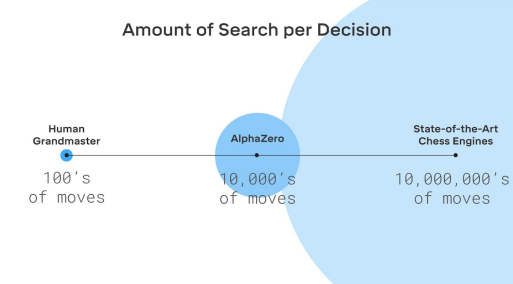
\includegraphics{Figures/A0 image.png}
\caption{A0 process comparison with other engines}
\label{fig:A0} 
\end{figure}

\subsection{Stockfish}

Stockfish is currently the best performing engine, originally built upon the older model based on historic data sets, it has since been improved to incorporate NNs into its model. This has allowed it to become relevant once again as the best publicly available chess engine \cite{popularChessEngines} as it consistently emerges victorious in the world computer chess championship (WCCC) among other competitions.

\subsection{Leela Chess Zero}

Lc0 is a top-performing chess engine that has gained popularity in recent years \cite{popularChessEngines}. It was built upon an open-source engine and utilizes crowd-sourced training, where individuals offer their hardware to help train the engine by running games that add to the dataset. As a result, Lc0 learns entirely on its own in an unsupervised fashion.

The abundance of historic data of top-level chess games dating back around 100 years is extremely useful as it shows the evolution of chess through the years as the average skill level improved with the newly available resources. In addition, numerous data sets available publicly include the millions of games played monthly on sites like Chess.com and Lichess.com. To break away from any patterns it may have formed during a particular training session, engines such as Lc0 have periodic datasets spanning six months each. These datasets are used to train individual neural networks (NNs), which are then incorporated into one single model. This helps Lc0 improve and adapt its play style to the changing trends and patterns in chess. \footnote{\url{https://github.com/LeelaChessZero/lczero-training}} \footnote{\url{https://storage.lczero.org/files/training_data/}}

\subsection{Maia}

A past study implemented Maia, a chess engine based on AlphaZero specifically tailored for predicting human moves \cite{SuperAI}. Saumik et al proposed a new approach to improve the strength of chess engines by incorporating human-like decision-making processes \cite{maia}. The authors argue that current chess engines lack the ability to make human-like decisions, which can lead to suboptimal moves and missed opportunities. To address this issue, they propose a new model that combines deep reinforcement learning with a human-like decision-making process.

The proposed model, called Hill-Climbing Policy Gradient (HCPG), is designed to learn from both human and computer-generated games. The model is trained to predict the moves made by human players and then uses these predictions to generate its own moves. The authors show that the HCPG model outperforms existing chess engines in terms of both win rate and human-like decision-making.

\section{Identifying the player}

From fingerprint sensors to unlock your phone, to maintaining a logged in account through cookies on your browser, there is an ever increasing number of applications seeking to know our identity, in most cases sacrificing security for convenience. Fingerprint sensors are common enough to be found on everyday phones \cite{fingerprint} and provide a way to add a security layer to a phone while being more convenient than traditional PIN or password locks. 

Having a chess engine learn to identify the user based on their pattern of play remains questionable, is it enough information to reliably deduce the identity of the player?

In recent years, there has been growing interest in using machine learning algorithms to identify players based on their pattern of play in games such as chess. Researchers have explored various approaches, ranging from analyzing move choices and timing to examining mouse movement and typing behavior.


///// Citations needed
While these methods show promise, their reliability and effectiveness in identifying players remains an open question. For instance, a study in 2019 found that the accuracy of player identification based on move choices alone ranged from 44 percent to 85 percent depending on the game and dataset used. Other studies have suggested that mouse movement and typing behavior may be more informative in identifying players, but also face challenges such as individual differences in motor skills and hardware variability.

/////////////////

The potential benefits of player identification in games are many, from enhancing security in online gaming to personalized game recommendations and learning. However, it is clear that more research is needed to develop accurate and reliable methods for identifying players based on their play, while also addressing concerns about privacy and ethical considerations.

\begin{figure}[ht]
\centering
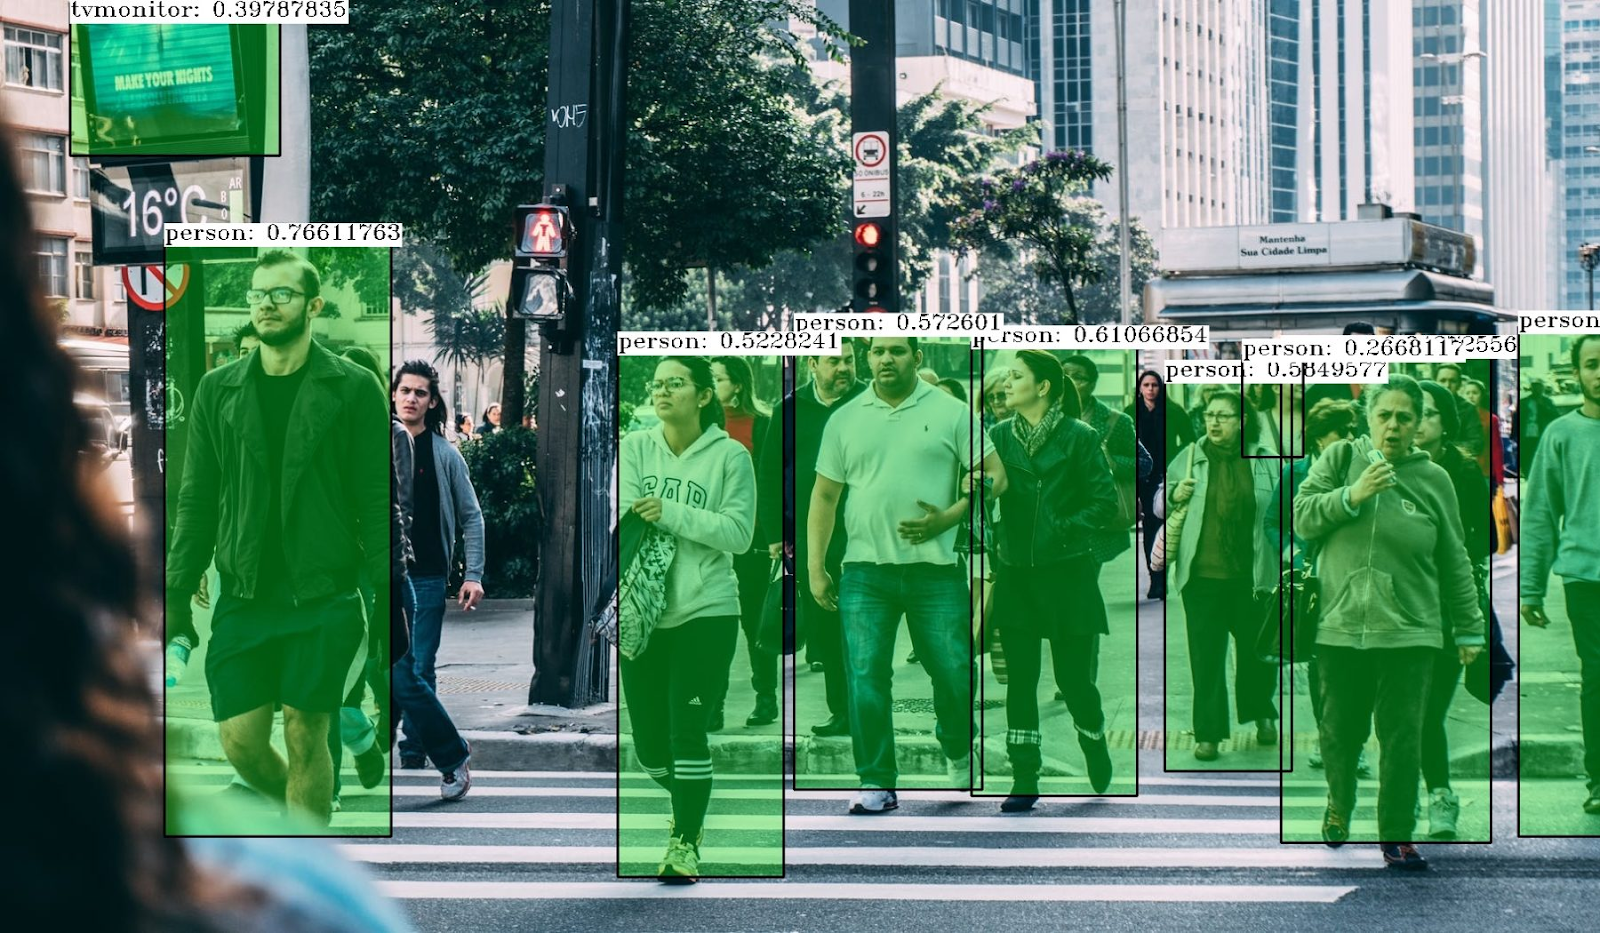
\includegraphics[width=5in, fbox]{Figures/opencv.png}
\caption{Machine Learning.}
\label{fig:opencvexample} 
\end{figure}

%=== END OF CHAPTER TWO ===
\end{spacing}
\newpage
